\documentclass[14pt]{extreport}
\usepackage{gost}

\newcommand{\ov}{\overline}
\newcommand{\fr}{\cfrac}
\newcommand{\ti}{\times}
\newcommand{\ttt}{\theta}
\newcommand{\wt}{\widetilde}

\newcommand{\lwo}{\widetilde{\overline{\lambda}}}%лямбда волна черта
\newcommand{\lw}{\overline{\lambda}}%лямбда черта
\newcommand{\lo}{\lambda_{0}}%лямбда о
\newcommand{\lnw}{\overline{\lambda}_{\nu}} %лямбда ню черта

\newcommand{\mwo}{\widetilde{\overline{\mu}}} %мю волна черта
\newcommand{\mw}{\overline{\mu}} %мю черта
\newcommand{\mo}{\mu_{\o}} %мю  о
\newcommand{\mnw}{\overline{\mu}_{\nu}} %мю ню черта

\newcommand{\ow}{\overline{\omega}}%омега черта

\newcommand{\rw}{\overline{r}}%r черта
\newcommand{\rrw}{\overline{r'}}%r' черта

\newcommand{\ew}{\overline{e}}%e черта
\newcommand{\vw}{\overline{v}}%v черта

\newcommand{\pw}{\overline{\rho}}%rho черта
\newcommand{\ppw}{\overline{\rho'}}%rho' черта

\newcommand{\Dt}{\Delta t}%delta t

\renewcommand{\phi}{\varphi} %нормальная фи

\begin{document}
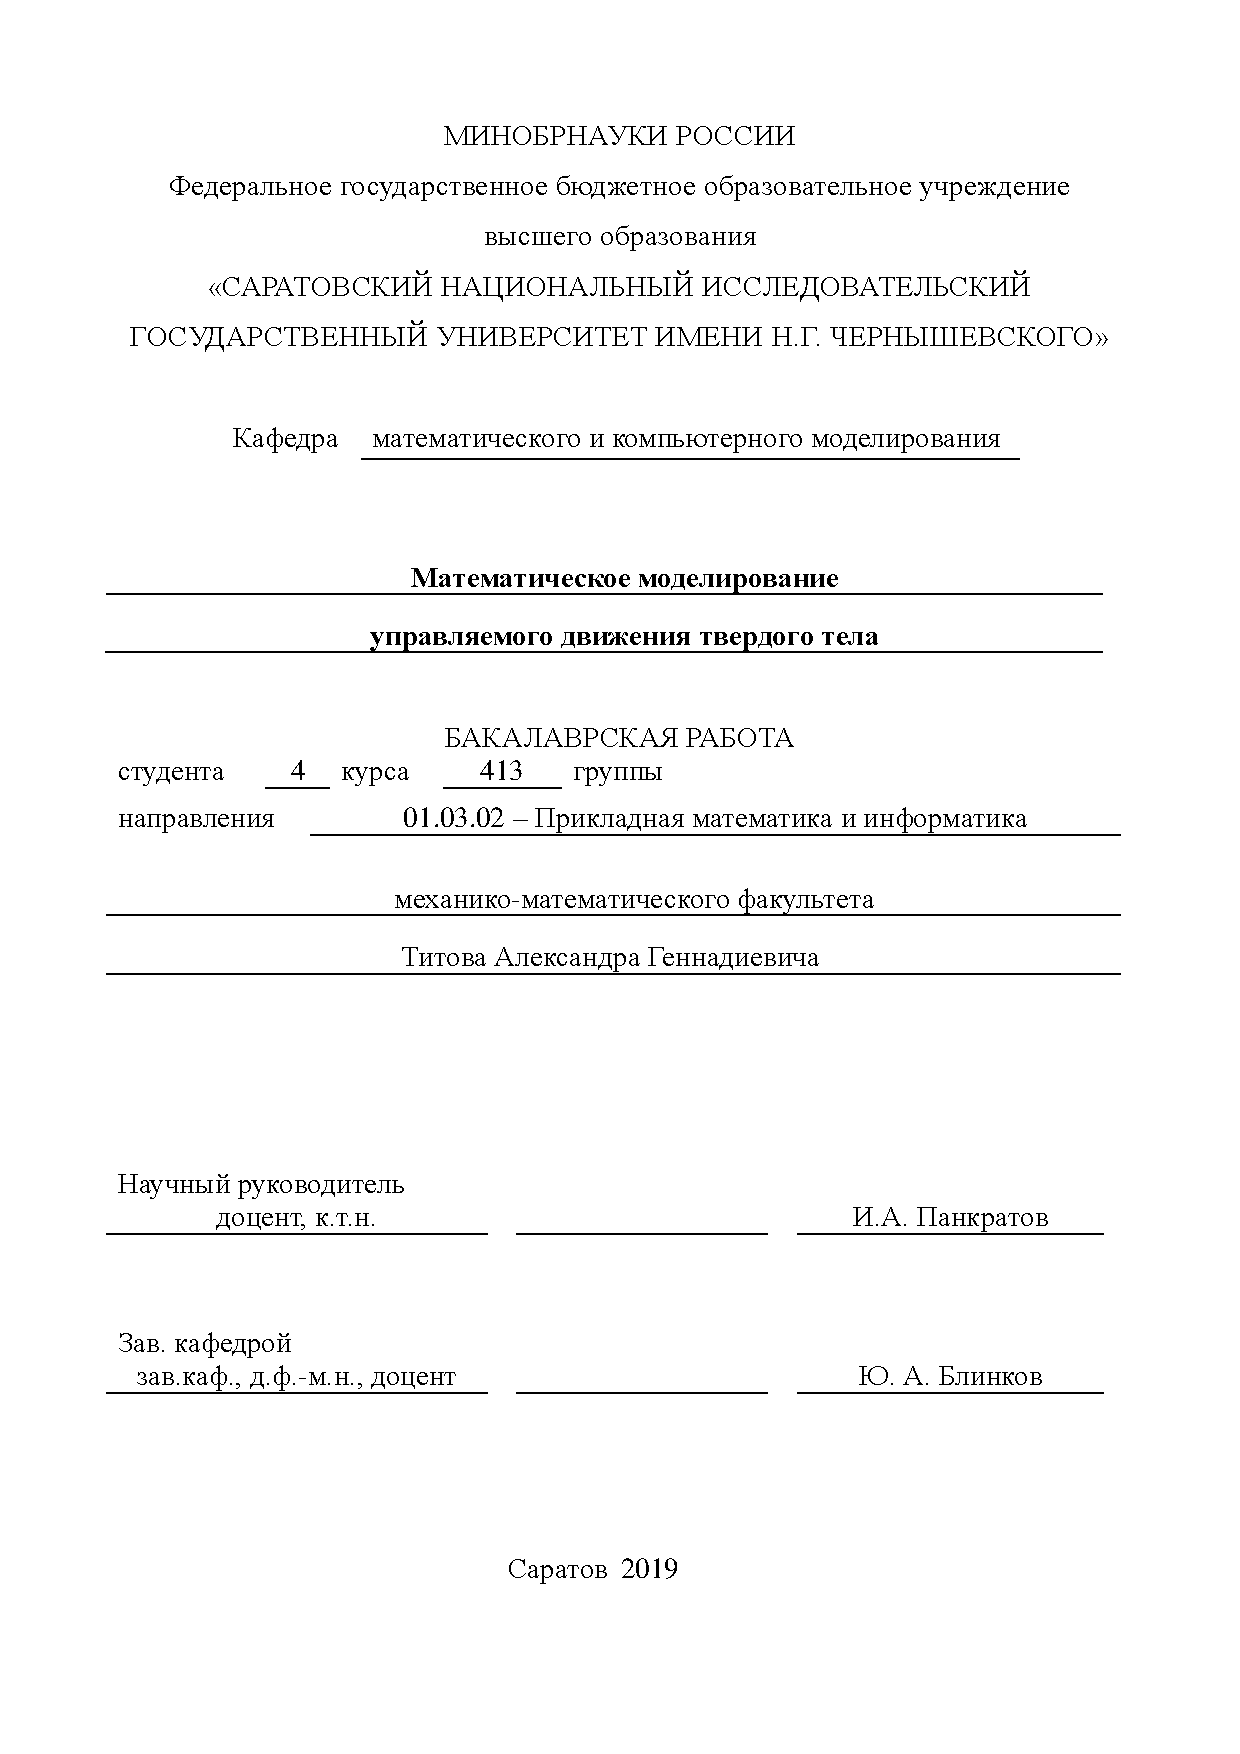
\includepdf[pages={1}]{titulDiplom.pdf}

\tableofcontents

\intro

Создание в середине 50-х годов прошлого столетия математической теории оптимального управления было связано с потребностями решения технических и экономических задач. Проблемы управления, в частности проблемы отыскания наилучшего, оптимального управления, возникают всюду. Наиболее яркие примеры таких задач – это задачи управления летательными аппаратами, управления технологическим процессом на производстве и т. п. В настоящее время оптимальное управление выросло в обширную самостоятельную теорию, использующую в своих исследованиях аппарат высшей алгебры, математического и функционального анализа, дифференциальных уравнений \cite{latex}.

Задачи оптимального управления относятся к самым сложным экстремальным задачам. Наиболее эффективным методом исследования этих задач является принцип максимума Понтрягина, представляющий собой необходимое условие оптимальности. Это одно из крупных достижений современной математики, которое обобщает и развивает основные результаты классического вариационного исчисления. Принцип максимума был сформулирован академиком Л.С. Понтрягиным в 1953 г. и в дальнейшем был доказан и развит им вместе с коллективом учеников и сотрудников.

За разработку теории оптимального управления Л.С. Понтрягину и его сотрудникам В.Г. Болтянскому, Р.В. Гамкрелидзе, и Е.Ф. Мищенко в 1962 году была присуждена Ленинская премия.

Целью бакалаврской работы является изучение задачи оптимальной переориентации твердого тела. Задано кватернионным дифференциальным кинематическим уравнением угловое движение твердого тела. Требуется изучить графики оптимального управления с разными весовыми множителями, которые переводят твердое тело из начального углового положения в конечное положение.

В первом разделе рассматриваем математические модели углового движения твердого тела, такие как: формула Родрига с конечным поворотом твердого тела с неподвижной точкой и кинематические уравнения Эйлера.

Во втором разделе - алгебра кватернионов, а именно основные операции над ними: сложение, умножение, деление, сопряженный и обратный кватернионы, норма и представление кватерниона в тригонометрической форме с помощью формулы Муавра.

В третьем разделе сначала рассматриваем общую задачу оптимального управления и применение принципа Л.С. Понтрягина.

В четвертом - постановка задачи для контретного кватернионного дифференциального кинематического уравнения.

В пятом - решение задачи оптимальной переориентации твердого тела путем сведение её к краевой задачи для системы обыкновенных дифференциальных уравнений с помощью принципа максимума.

В шестом, седьмом и восьмом разделах - разработка численного решения задачи с базой данных для хранения результатов проведённых экспериментов.

\chapter{Математические модели углового движения твердого тела}
\section{Формула Родрига. Конечный поворот твердого тела с неподвижной точкой}

Рассмотрим твердое тело с одной неподвижной точкой $O$. Телу сообща­ется поворот вокруг оси, задаваемой единичным вектором $e$, на угол $\phi$. Направление вектора $e$ выбирается так, чтобы, смотря с его конца, видеть поворот тела на угол, меньший или равный $180^{\circ}$, происходящий против хода часовой стрелки \cite{chelnokov}.

Рассмотрим произвольную точку твердого тела, занимающую до по­ворота тела положение $M$, а после поворота — положение $M'$, изображенная в соответствии с рисунком 1.1.

\begin{figure}[H]
\center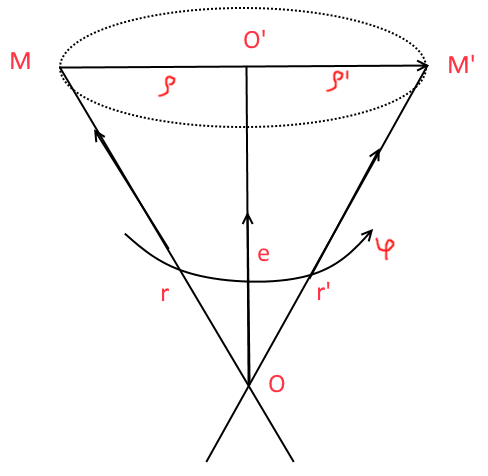
\includegraphics[scale=0.5]{fig/img11.png}
\caption{Конечный поворот твердого тела}
\end{figure}

Радиус-вектор точки до поворота $\overline{OM}=r$. После поворота он займет положение $\overline{OM'}=r'$, так что вектор $\overline{MM'}=r'-r$ представляет собой вектор перемещения точки $M$ при повороте тела. Это перемещение требуется выразить через величины (угол $\phi$ и вектор $e$), определяю­щие поворот, и вектор $r$(то есть, требуется найти зависимость $r' = f(r, e,\phi)$).

Очевидно, что векторы $r$ и $r'$ определяются равенствами
\begin{equation}
r = \overline{OO'} + \rho,\ r' = \overline{OO'} + \rho'
\end{equation}
и являются образующими кругового конуса, по оси которого направлен единичный вектор $e$.

Составляющая $\overline{OO'}$ вектора $r$, направленная вдоль оси поворота, не изменяется при повороте:
\begin{equation}
\overline{OO'} = re = r'e,
\end{equation}
поэтому остается проследить за изменением составляющей, перпенди­кулярной оси поворота,
\begin{equation}
\label{rho1}
\rho=r-(re)e,
\end{equation}
переходящей в вектор
\begin{equation}
\label{rho2}
\rho'=r'-(r'e)e=r'-(re)e.
\end{equation}

В соответствие с рисунком 1.1 следует, что
\begin{equation}
\ppw = \ov{O'S} + \ov{SM'} = \fr{1}{2}(\pw + \ppw)+\ov{SM'},
\end{equation}
где $S$ — точка, делящая отрезок $MM'$ пополам.

Заметив, что вектор
\begin{equation}
\ov{SM'} = \tg(\fr{\phi}{2})(\ew\ti\ov{O'S}) = \fr{1}{2} \tg(\fr{\phi}{2})(e\times(\pw+\ppw)),
\end{equation}
получим
\begin{equation}
\ppw = \fr{1}{2}(\pw+\ppw) + \fr{1}{2}\tg(\fr{\phi}{2})\ew\ti(\pw+\ppw)
\end{equation}
или
\begin{equation}
\ppw - \tg(\fr{\phi}{2})\ew\ti\ppw = \pw + \tg(\fr{\phi}{2})\ew\ti\pw.
\end{equation}

Подставляя в это равенство выражения для $\rho$ и $\rho'$ из \eqref{rho1} и \eqref{rho2}, придем к формуле
\begin{equation}
\rrw - \tg(\fr{\phi}{2})\ew\ti\rrw = \rw + \tg(\fr{\phi}{2})\ew\ti\rw.
\end{equation}

Остается разрешить это уравнение относительно $r'$, для этого умно­жим обе его части векторно слева на $e$. Тогда придем к уравнению
\begin{equation}
\label{relat-r}
\ov{e}\ti\ov{r'} - \tg(\fr{\phi}{2})[\ov{e}(\ov{e}\ov{r'})-\ov{r'}] = \ov{e}\ti\ov{r} - \tg(\fr{\phi}{2})[\ov{e}(\ov{e}\ov{r})-\ov{r}].
\end{equation}

Исключив из этого уравнения вектор $e \times r'$ с помощью \eqref{relat-r}, получим
\begin{equation}
\label{relat-r2}
\ov{r'} = \ov{r}[1+\fr{2tg^{2}(\fr{\phi}{2})}{(1+tg^{2}(\fr{\phi}{2}))} + \fr{2}{(1+tg^{2}(\fr{\phi}{2}))}[tg(\fr{\phi}{2})\ov{e}\ti\ov{r} + tg^{2}(\fr{\phi}{2})(\ov{e}\ov{r})\ov{e}].
\end{equation}

Введем в рассмотрение вектор $\theta=2 tg \dfrac{\phi}{2}e,$ называемый вектором конечного поворота. Тогда формула \eqref{relat-r2} примет вид:
\begin{equation}
\label{formula-Rodrig}
\ov{r'} = \ov{r} + (1+ \fr{\ov{\theta}^{2}}{4})^{-1}[\ov{\ttt}\ti(\ov{r}+\fr{\ov{\ttt}}{2}\ti\ov{r})].
\end{equation}

Эта формула называется формулой Родрига. Ее можно записать в дру­гом виде:
\begin{equation}
\label{form-Rodrig2}
\ov{r'} = \ov{r} + sin\phi(\ov{e}\ti\ov{r}) + (1 - cos\phi)(\ov{e}\ti(\ov{e}\ti\ov{r}))
\end{equation}
или
\begin{equation}
\label{form-Rodrig3}
\ov{r'} = cos\phi\ov{r} + sin\phi(\ov{e}\ti\ov{r}) + (1 - cos\phi)(\ov{e}\ov{r})\ov{e}.
\end{equation}

Полученные формулы \eqref{formula-Rodrig}, \eqref{form-Rodrig2}, \eqref{form-Rodrig3} связывают радиусы-векторы произвольной точки твердого тела, имеющего одну неподвижную точку, до поворота тела и после поворота с величинами $\phi$ и $e$ (эйлеровым углом поворота и единичным вектором эйлеровой оси поворота), характери­зующими конечный поворот твердого тела в пространстве.

\section{Кинематические уравнения Эйлера}
Будем считать, что точка $O$ твердого тела неподвижна, и что систе­ма координат $Y$, жестко связанная с телом, совпадала в его начальном положении с опорной системой координат $X$. Тогда твердое тело может быть переведено из этого начального положения в любое конечное положение с помощью трех поворотов на углы Эйлера: прецессии $\psi$, нутации $\vartheta$ и собственного вращения $\phi$, изображены в соответствии с рисунком 1.2.

\begin{figure}[H]
\center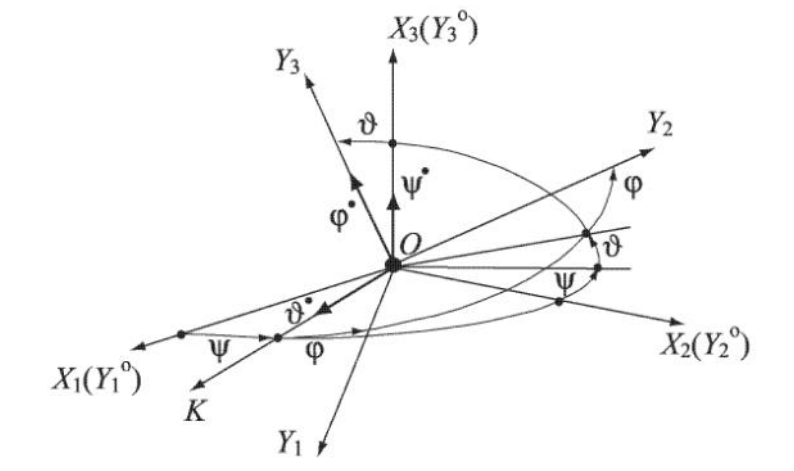
\includegraphics[scale=0.5]{fig/img12.png}
\caption{Углы Эйлера: $\psi$, $\vartheta$ и $\phi$}
\end{figure}

Рассмотрим два положения твердого тела: первое определяется значениями $\psi,\ \vartheta,\ \phi$ эйлеровых углов, второе, бесконечно близкое к первому, их значениями $\phi+\delta\phi,\ \vartheta+\delta\vartheta,\ \psi+\delta\psi$. Переход из первого положения во второе можно осуществить с помощью трех бесконечно малых поворотов, определяемых векторами
\begin{equation}
\delta\psi=\delta\psi x_{3},\ \delta\vartheta=\delta\vartheta y_{1}',\ \delta\phi=\delta\phi y_{3}.
\end{equation}

Здесь $\delta\phi,\ \delta\vartheta,\ \delta\psi$ — углы бесконечно малых поворотов; $x_{3},\ y_{1}', y_{3}$ — единичные векторы осей прецессии, нутации и собственного вращения (осей $OX_{3},\ OK,\ OY_{3}$).

Вектор $\delta\theta$ результирующего бесконечно малого поворота равен гео­метрической сумме векторов слагаемых поворотов:
\begin{equation}
\delta\theta=\delta\psi+\delta\vartheta+\delta\phi=\delta\psi x_{3}+\delta\vartheta y_{1}'+\delta\phi y_{3}.
\end{equation}

Из этого равенства следует
\begin{equation}
\delta\phi=(\phi^{\cdot} x_{3})dt,\ \delta\vartheta=(\vartheta^{\cdot} y_{1}')dt,\ \delta\psi=(\psi^{\cdot} y_{3})dt,
\end{equation}
связывающих векторы бесконечно малых поворотов с мгновенными угловыми скоростями элементарных (отдельных) поворотов, получим выражение для вектора мгновенной угловой скорости твердого тела:
\begin{equation}
\label{res-omega}
\omega=\phi^{\cdot} x_{3}+\vartheta^{\cdot} y_{1}'+\psi^{\cdot} y_{3}.
\end{equation}

Приведем другое, более простое, доказательство формулы \eqref{res-omega}. Положение (движение) твердого тела с одной неподвижной точкой в пространстве можно однозначно характеризовать (задавать) тремя углами Эйлера, поэтому мгновенное движение такого тела можно представлять как композицию трех мгновенных плоских эйлеровых вращений (в любой последовательности) с мгновенными угловыми скоростями прецессии $\phi^{\cdot} x_{3}$, нутации $\vartheta^{\cdot} y_{1}'$ и собственного вращения $\psi^{\cdot} y_{3}$. Поскольку векторы этих угловых скоростей пересекаются в одной (неподвижной) точке $O$ тела, то в соответствии с теорией сложного движения твердого тела результирующее мгновенное движение твердого тела представляет собой мгновенное вращение с мгновенной угловой скоростью, определяемой формулой \eqref{res-omega}.

Проектируя векторное равенство \eqref{res-omega} на связанные координатные оси, получим связи проекций $\omega_{i}$ (i = 1,2,3) вектора мгновенной угло­вой скорости твердого тела с углами Эйлера и их первыми производ­ными по времени:
\begin{equation}
\label{omega-angular-Euler}
\begin{split}
\omega_{1}=\vartheta^{\cdot}\cos\phi+\psi^{\cdot}\sin\vartheta\sin\phi,\\
\omega_{2}=-\vartheta^{\cdot}\sin\phi+\psi^{\cdot}\sin\vartheta\cos\phi,\\
\omega_{3}=\phi+\psi^{\cdot}\cos\vartheta.
\end{split}
\end{equation}

Разрешая соотношения \eqref{omega-angular-Euler} относительно производных $\psi^{\cdot},\ \vartheta^{\cdot},\ \phi^{\cdot}$ получаем кинематические уравнения Эйлера, имеющие вид
\begin{equation}
\label{kinematic-eq-Euler}
\begin{split}
\psi^{\circ}=\dfrac{1}{\sin\vartheta}(\omega_1\sin\phi+\omega_2\cos\phi),\\
\\vartheta^{\circ}=\omega_1\cos\phi-\omega_2\sin\phi),\\
\phi^{\circ}=\omega_3-ctg\vartheta(\omega_1\sin\phi+\omega_2\cos\phi).
\end{split}
\end{equation}

Получим другую форму кинематических уравнений Эйлера. Для этого спроектируем векторное равенство \eqref{res-omega} на оси опорной (непо­движной) системы координат $X$. Обозначая через $\omega_i^{*}=\omega_i^{*}(t)$, (i = 1,2,3) проекции вектора $\omega$ мгновенной угловой скорости твердого тела на оси опорной системы координат, получим
\begin{equation}
\label{kinematic-eq-Euler2}
\begin{split}
\omega_{1}^{*}=\omega_3^{*}-ctg\vartheta(\omega_1^{*}\sin\psi-\omega_2^{*}\cos\psi),\\
\omega_{2}^{*}=\vartheta^{\circ}\sin\psi-\phi^{\circ}\sin\vartheta\cos\psi,\\
\omega_{3}^{*}=\psi^{\circ}+\phi^{\circ}\cos\vartheta.
\end{split}
\end{equation}

Разрешая соотношения \eqref{kinematic-eq-Euler2} относительно производных $\psi^{\cdot},\ \vartheta^{\cdot},\ \phi^{\cdot}$, получим другую форму кинематических уравнений Эйлера, связыва­ющих проекции $\omega_{i}^{*}$ (i = 1,2,3) вектора мгновенной угловой скорости твердого тела на оси опорной системы координат с углами Эйлера и их первыми производными по времени:
\begin{equation}
\label{kinematic-eq-Euler3}
\begin{split}
\psi^{\circ}=\omega_3^{*}-ctg\vartheta(\omega_1^{*}\sin\psi-\omega_2^{*}\cos\psi),\\
\vartheta^{\circ}=\omega_1^{*}\cos\psi+\omega_2^{*}\sin\psi,\\
\phi^{\circ}=\dfrac{1}{\sin\vartheta}(\omega_1^{*}\sin\psi-\omega_2^{*}\cos\psi).
\end{split}
\end{equation}

Уравнения \eqref{kinematic-eq-Euler} и \eqref{kinematic-eq-Euler3} в случаях, когда $\omega_{i}=\omega_{i}(t)$ (i = 1,2,3) или когда $\omega_{i}^{*}=\omega_{i}^{*}(t)$, т. е. когда проекции вектора мгновенной угловой скорости твердого тела на связанные с ним координатные оси или на оси опорной системы координат являются известными функциями времени, образуют системы нелинейных нестационарных дифференци­альных уравнений третьего порядка относительно углов Эйлера $\psi,\ \vartheta,\ \phi$. Эти системы имеют особую точку $\vartheta=0$, в которой кинематические уравнения Эйлера вырождаются.

Отметим, что существование особой точки $\vartheta=0$ в уравнениях движения твердого тела с одной неподвижной точкой в большинстве случаев не связано с физикой движения твердого тела, а обуслов­лено выбранным нами способом описания движения твердого тела, и, следовательно, от этой особой точки можно избавиться за счет использования другого способа описания движения (например, за счет использования в качестве кинематических параметров направляющих косинусов углов или параметров Эйлера). Исключение составляет слу­чай, когда неподвижная точка твердого тела материализуется с помо­щью трехосного карданова подвеса, реализующего повороты твердого тела на углы Эйлера. В этом случае особая точка $\vartheta=0$ отвечает эффекту складывания рам карданова подвеса, при котором твердое тело теряет одну степень свободы.

\chapter{Алгебра кватернионов}
Под кватернионом понимают число, составленное из действительной единицы 1 и трех мнимых единиц $i_{1}, i_{2}, i_{3},$ с действительными элементами следующего вида:
\begin{equation}
\label{quaternion-def}
\lambda = (\lambda_{0}, \lambda_{1}, \lambda_{2}, \lambda_{3}) = \lambda_{0} 1 + \lambda_{1} i_{1} + \lambda_{2} i_{2} + \lambda_{3} i_{3}.
\end{equation}

Изложим основ­ные правила, определяющие действия над кватернионами \cite{branets}.

\textbf{1. Равенство двух кватернионов.} Два кватерниона $\lambda$ и $\mu$ равны, если равны их элементы $\lambda_{j}$ и $\mu_{j}$, $j = \overline{0,3}$.

\textbf{2. Нулевой кватернион.} Нулевым называется кватернион, элементы которого нули.

\textbf{3. Сложение кватернионов.} Суммой кватернионов $\lambda$ и $\mu$ называется кватернион $v$ с элементами $\nu_{j} = \lambda_{j} + \mu_{j}, j = \overline{0,3}$:
\begin{equation}
\label{sum-quat}
\nu = \lambda + \mu = (\lambda_{0} + \mu_{0}) 1 + (\lambda_{0} + \mu_{0}) 1 + (\lambda_{1} + \mu_{1}) i_{1} + (\lambda_{2} + \mu_{2}) i_{2} + (\lambda_{3} + \mu_{3}) i_{3}.
\end{equation}

Сложение кватернионов подчиняется правилам обычной алгебры:
\begin{equation}
\label{sum-quat-algebra}
\lambda + \mu = \mu + \lambda,\ (\lambda + \mu)+\nu = \lambda + (\mu+\nu).
\end{equation}

\textbf{4. Умножение кватернионов.} При умножении кватерниона $\lambda$ на скаляр $a$ происходит умножение на это число всех его элементов:
\begin{equation}
\label{scal-mul-quat}
a\lambda=a\lambda_{0}1+a\lambda_{1}i_{1}+a\lambda_{2}i_{2}+a\lambda_{3}i_{3}.
\end{equation}

Умножение на скаляр подчиняется правилам обычной алгебры ($a,\ b$ — скаляры): $a\lambda = \lambda a,\ (ab)\lambda = \lambda(ab),\ (a + b)\lambda = a\lambda + b\lambda,\ a(\lambda + \mu) = a\lambda + a\mu.$

Единицы $1,\ i_{1},\ i_{2},\ i_{3}$ можно рассматривать как единичные векторы (орты) четырехмерного пространства. Тогда любой кватернион можно представить в этом пространстве точкой или радиусом-вектором. Сложение векторов и умножение их на скаляр в этом пространстве происходит так же, как и в обычном векторном пространстве.

Для того чтобы определить произведение кватернионов, необходимо задать правила умножения единиц $1,\ i_{1},\ i_{2},\ i_{3}$. Эти правила были введены Гамильтоном в 1843 г. и таковы:
\begin{equation}
\label{H-rules}
\begin{split}
1\circ 1 = 1,\ 1\circ i_{1} = i_{1} \circ 1 = i_{1},\ 1\circ i_{2} = i_{2} \circ 1 = i_{2},\ 1\circ i_{3} = i_{3} \circ 1 = i_{3},\\
i_{1}\circ i_{1} = -1,\ i_{2}\circ i_{2} = -1,\ i_{3}\circ i_{3} = -1,\\
i_{1}\circ i_{2} = -i_{2}\circ i_{1} = i_{3},\ i_{3}\circ i_{1} = -i_{1}\circ i_{3} = i_{2},\ i_{2}\circ i_{3} = -i_{3}\circ i_{2} = i_{1}.
\end{split}
\end{equation}

Здесь символ «$\circ$» означает кватернионное умножение.

При таких правилах умножения кватернионных единиц произведение двух кватернионов также является кватернионом.

Правила умножения кватернионных единиц легко запомнить, если использовать следующую схему, изображенная в соответствии с рисунком 2.1.
\begin{figure}[h]
\center 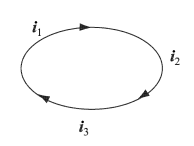
\includegraphics[scale=1]{fig/img21.png}
\caption{Правило умножения кватернионных единиц}
\end{figure}

При умножении двух единиц, расположенных по ходу часовой стрелки, получается третья единица с плюсом; при расположении единиц в обратном порядке (против хода часовой стрелки) получается третья единица со знаком минус. Правила умножения чрезвычайно удобны — благодаря им алгебра кватернионов содержит в себе алгебру действительных и комплексных чисел, а также трехмерную векторную алгебру. Кватернионы содержат действительные числа $(a,0,0,0)$ с единственной единицей $1$, комплексные числа $(a,b,0,0)$ с двумя единицами $1,\ i$ и векторы $(0, a, b, c)$ с ортами $i_{1},i_{2},i_{3}$ трехмерного векторного пространства.

Кватернионные единицы $i_{1},\ i_{2},\ i_{3}$ можно совместить с ортами трехмерного векторного пространства и рассматривать коэффициенты при этих единицах как компоненты вектора. В соответствии с этим кватернион $\lambda$ можно представить в виде скалярной $\lambda_{0}$ и векторной $\lambda_{\nu}$ частей:
\begin{equation}
\label{quat-sum-scal-vect}
\lambda=\lambda_{0}+\lambda_{\nu},\ \lambda_{\nu}=\lambda_{1}i_{1}+\lambda_{2}i_{2}+\lambda_{3}i_{3}.
\end{equation}

Используя это представление и правила умножения кватернионных единиц \eqref{H-rules}, произведение двух кватернионов $\lambda,\ \mu$ можно представить (используя операции векторной алгебры) в следующем виде:
\begin{equation}
\label{quat-mul-quat}
\begin{split}
\lambda \circ \mu = \lambda_{0}\mu_{0}-\lambda_{1}\mu_{1}-\lambda_{2}\mu_{2}-\lambda_{3}\mu_{3}+\lambda_{0}(\mu_{1}i_{1}+\mu_{2}i_{2}+\mu_{3}i_{3})+\\
+\mu_{0}(\lambda_{1}i_{1}+\lambda_{2}i_{2}+\lambda_{3}i_{3})+
\begin{vmatrix}
  i_{1}\ i_{2}\ i_{3}\\
  \lambda_{1}\ \lambda_{2}\ \lambda_{3}\\
  \mu_{1}\ \mu_{2}\ \mu_{3}
\end{vmatrix} =\\
= \lambda_{0}\mu_{0}-\lambda_{\nu}\mu_{\nu}+\lambda_{0}\mu_{\nu}+\lambda_{\nu}\mu_{0}+\lambda_{\nu}\times \mu_{\nu}.
\end{split}
\end{equation}

Отсюда видно, что если поменять местами сомножители, т. е. рассматривать произведение $\mu \circ \lambda$, то в формуле \eqref{quat-mul-quat} изменится знак детерминанта. Следовательно, умножение кватернионов некоммутативно: $\lambda \circ \mu \neq \mu \circ \lambda$.

Перестановка сомножителей допустима лишь тогда, когда один из сомножителей является скалярным или когда векторные части сомножителей пропорциональны.

Из формулы \eqref{quat-mul-quat} также следует, что в результате кватернионного умножения векторов получается не вектор, а кватернион:
\begin{equation}
\label{res-quat-mul}
\lambda_{\nu} \circ \mu_{\nu} = -\lambda_{\nu} \mu_{\nu} + \lambda_{\nu} \times \mu_{\nu}
\end{equation}

Из формулы \eqref{res-quat-mul} видно, что понимаемое в обычной векторной алгебре скалярное и векторное произведения двух векторов равны соответственно скалярной части кватернионного произведения этих векторов, взятой со знаком минус, и векторной части кватернионного произведения:
\begin{equation}
\lambda_{\nu}\mu_{\nu} = -scal(\lambda_{\nu} \circ \mu_{\nu}),\ \lambda_{\nu} \times \mu_{\nu} = vect(\lambda \circ \mu).
\end{equation}

Используя правила \eqref{H-rules}, можно доказать, что умножение кватернионов обладает ассоциативными и дистрибутивными по отношению к сложению свойствами:
\begin{equation}
(\lambda \circ \mu) \circ \nu = \lambda \circ ( \mu \circ \nu),\ \lambda \circ (\mu + \nu) = \lambda \circ  \mu + \lambda \circ \nu.
\end{equation}

Напомним, что векторное произведение векторов ассоциативным свойством не обладает.

Для скалярной и векторной частей кватернионого произведения двух векторов справедливы соотношения
\begin{equation}
\begin{split}
scal(\lambda_{\nu} \circ \mu_{\nu}) = scal(\mu_{\nu} \circ \lambda_{\nu}), vect(\lambda_{\nu} \circ \mu_{\nu}) = -vect(\mu_{\nu} \circ \lambda_{\nu}),\\
scal(\lambda_{\nu} \circ \mu_{\nu}) = -\lambda_{\nu} \mu_{\nu} = \dfrac{1}{2}(\lambda_{\nu} \circ \mu_{\nu}+ \mu_{\nu} \circ \lambda_{\nu}),\\
vect(\lambda_{\nu} \circ \mu_{\nu}) = \lambda_{\nu} \times \mu_{\nu} = \dfrac{1}{2}(\lambda_{\nu} \circ \mu_{\nu}- \mu_{\nu} \circ \lambda_{\nu}).
\end{split}
\end{equation}

Отметим также следующие свойства скалярных частей произведений кватернионов:
\begin{equation}
\begin{split}
scal(\lambda \circ \mu) = scal(\mu \circ \lambda),\\
scal(\lambda \circ \mu \circ \nu) = scal(\mu \circ \nu \circ \lambda) = scal(\nu \circ \lambda \circ \mu),
\end{split}
\end{equation}
т. е. скалярная часть произведения кватернионов не меняется при циклической перестановке сомножителей.

Пусть даны два кватерниона $\lambda$ и $\mu$ и пусть кватернион $\nu$ определяется как произведение кватернионов $\lambda$ и $\mu$:
\begin{equation}
\label{res-quat-mul-quat}
\nu = \lambda \circ \mu.
\end{equation}

Используя формулу \eqref{quat-mul-quat}, из \eqref{res-quat-mul-quat} получим выражения компонент кватерниона $\nu$ через компоненты кватернионов $\lambda$ и $\mu$:
\begin{equation}
\label{nu-lambda-mu}
\begin{split}
\nu_{0}=\lambda_{0}\mu_{0}-\lambda_{1}\mu_{1}-\lambda_{2}\mu_{2}-\lambda_{3}\mu_{3},\\
\nu_{1}=\lambda_{0}\mu_{1}+\lambda_{1}\mu_{0}+\lambda_{2}\mu_{3}-\lambda_{3}\mu_{2},\\
\nu_{2}=\lambda_{0}\mu_{2}-\lambda_{1}\mu_{3}+\lambda_{2}\mu_{0}+\lambda_{3}\mu_{1},\\
\nu_{3}=\lambda_{0}\mu_{3}+\lambda_{1}\mu_{2}-\lambda_{2}\mu_{1}+\lambda_{3}\mu_{0}.
\end{split}
\end{equation}


\textbf{5. Сопряженный кватернион.} Кватернионом, сопряженным данному кватерниону $\lambda$, является кватернион, обозначаемый $\overline{\lambda}$ и определяемый формулой $\overline{\lambda}=\lambda_{0}-\lambda_{1}i_{1}-\lambda_{2}i_{2}-\lambda_{3}i_{3}=\lambda_{0}-\lambda_{\nu}$.

Сопряженные сумме и произведению двух кватернионов находятся
по формулам
\begin{equation}
\label{linked-sum-mul}
(\overline{\lambda+\mu})=\overline{\lambda}+\overline{\mu},\ (\overline{\lambda\circ\mu})=\overline{\lambda}\circ\overline{\mu}.
\end{equation}

По индукции свойства \eqref{linked-sum-mul} легко доказываются для случаев $n$ кватернионных слагаемых и $n$ сомножителей.

\textbf{6. Норма кватерниона.} Нормой кватерниона $\lambda$ называется величина 
\begin{equation}
||\lambda|| = \lambda \circ \overline{\lambda} = \overline{\lambda} \circ \lambda = \lambda_{0}^{2}+\lambda_{1}^{2}+\lambda_{2}^{2}+\lambda_{3}^{2}.
\end{equation}

Если норма кватерниона равна 1 ($||\lambda|| = 1$), то кватернион называется нормированным или единичным \cite{demidovich}.

Норма произведения кватернионов равна произведению норм сомножителей: 
\begin{equation}
||\lambda_{1} \circ \lambda_{2} \circ \dots \circ \lambda_{n}|| = ||\lambda_{1}||\ ||\lambda_{2}|| \dots ||\lambda_{n}||.
\end{equation}

\textbf{7. Деление кватернионов. Обратный кватернион.} Пусть кватернион $\nu$ является произведением кватернионов $\lambda$ и $\mu$:
\begin{equation}
\label{res-nu-mul-lambda-mu}
\nu=\lambda \circ \mu
\end{equation}

И пусть необходимо определить по заданным $\nu$ и $\lambda$ ($\nu$ и $\mu$) кватернион $\mu$($\lambda$). Для этого необходимо определить операцию деления кватернионов. В координатах эта операция равносильна решению системы линейных неоднородных алгебраических уравнений \eqref{nu-lambda-mu} относительно неизвестных $\mu_{j}$ или $\lambda_{j},\ j=\overline{0,3}.$

С операцией деления кватернионов тесно связано понятие обратного кватерниона: кватернионом, обратным данному кватерниону $\lambda$, называется кватернион $\lambda^{-1}$, определяемый формулой
\begin{equation}
\lambda^{-1}=||\lambda||^{-1}\overline{\lambda}.
\end{equation}

Для обратного кватерниона справедливо равенство
\begin{equation}
\lambda \circ \lambda^{-1} = \lambda^{-1} \circ \lambda = 1.
\end{equation}

Исходя из этого понятия, уравнение \eqref{res-nu-mul-lambda-mu} можно решить относительно неизвестного кватерниона $\lambda$ следующим образом: умножим справа данное уравнение на $\nu^{-1}$, в результате получим
\begin{equation}
\label{relat-lambda}
\lambda = \nu \circ \mu^{-1} = ||\mu||^{-1} \nu \circ \overline{\mu}.
\end{equation}

Для случая неизвестного $\mu$ получаем аналогично:
\begin{equation}
\label{relat-mu}
\mu = \lambda^{-1} \circ \nu = ||\lambda||^{-1} \lambda \circ \nu.
\end{equation}

Формулы \eqref{relat-lambda} и \eqref{relat-mu} определяют операцию деления кватернионов и являются решениями уравнения \eqref{res-nu-mul-lambda-mu}. Некоммутативность умножения кватернионов приводит к несимметричным формулам для нахождения кватернионов $\lambda$ и $\mu$.

Кватернион, обратный произведению кватернионов, находится следующим образом:
\begin{equation}
(\lambda_{1} \circ \lambda_{2} \circ \dots \circ \lambda_{n})^{-1} = \lambda_{n}^{-1} \circ \lambda_{n-1}^{-1}\circ \dots \circ \lambda_{2}^{-1}\circ \lambda_{1}^{-1}.
\end{equation}

\textbf{Представление кватерниона в тригонометрической форме. Формула Муавра.} Любой кватернион $\lambda = \lambda_{0} + \lambda_{1}i_{1} + \lambda_{2}i_{2} + \lambda_{3}i_{3} = \lambda_{0} + \lambda_{\nu}$ с действительными элементами $\lambda_{j}, j = \overline{0,3}$ может быть представлен в следующем виде:
\begin{equation}
\label{quat-lambda}
\lambda = \lambda \Bigl( \dfrac{\lambda_{0}}{\lambda} + \dfrac{\lambda_{1}i_{1}+\lambda_{2}i_{2}+\lambda_{3}i_{3}}{\lambda} \Bigl) = \lambda \Bigl( \dfrac{\lambda_{0}}{\lambda} + \dfrac{\lambda_{\nu}}{\lambda} \Bigl),
\end{equation}
где величина
\begin{equation}
\lambda = (\lambda_{0}^{2}+\lambda_{1}^{2}+\lambda_{2}^{2}+\lambda_{3}^{2})^{1/2} = ||\lambda||^{1/2} = |\lambda|
\end{equation}
называется тензором данного кватерниона.

Очевидно, что тензор нормированного (единичного) кватерниона равен единице. Величина
$$\dfrac{\lambda_{0}}{\lambda} + \dfrac{\lambda_{\nu}}{\lambda}$$
называется верзором кватерниона, т. е. верзор — кватернион, норма которого равна единице. Это название связано с тем, что вращение может быть задано с помощью единичного кватерниона.

Введем единичный вектор $\xi$, направленный вдоль вектора $\lambda_{\nu}$:
\begin{equation}
\xi=\dfrac{\lambda_{\nu}}{(\lambda_{1}^{2}+\lambda_{2}^{2}+\lambda_{3}^{2})^{1/2}}=\dfrac{\lambda_{1}i_{1} + \lambda_{2}i_{2} + \lambda_{3}i_{3}}{(\lambda_{1}^{2}+\lambda_{2}^{2}+\lambda_{3}^{2})^{1/2}}.
\end{equation}

Тогда векторная часть верзора может быть записана в таком виде:
\begin{equation}
\label{vect-part-verzor}
\dfrac{\lambda_{\nu}}{\lambda}=\dfrac{(\lambda_{1}^{2}+\lambda_{2}^{2}+\lambda_{3}^{2})^{1/2}}{\lambda}\xi.
\end{equation}

Замечая, что сумма квадратов скалярной части верзора и коэффициента при $\xi$ в \eqref{vect-part-verzor} равна единице, введем следующие переменные:
\begin{equation}
\cos v=\dfrac{\lambda_{0}}{\lambda},\ \sin v=\dfrac{(\lambda_{1}^{2}+\lambda_{2}^{2}+\lambda_{3}^{2})^{1/2}}{\lambda},\ 0\leq v \leq \pi.
\end{equation}

С учетом этих обозначений кватернион \eqref{quat-lambda} может быть представлен в следующем виде:
\begin{equation}
\label{quat-trig}
\lambda=\lambda(\cos v + \xi \sin v).
\end{equation}

Представление кватерниона в тригонометрической форме \eqref{quat-trig} удобно тем, что позволяет легко находить корни уравнения. Действительно, поскольку $\xi \circ \xi = -\xi \xi + \xi \times \xi = -\xi \xi = -1,$ то
\begin{equation}
\lambda^{2}=\lambda \circ \lambda = \lambda^{2}(\cos v + \xi \sin v) \circ (\cos v + \xi \sin v) = \lambda^{2}(\cos (2v)+\xi \sin(2v))
\end{equation}
и для любой степени $n$ справедлива формула Муавра \cite{matan}:
\begin{equation}
\lambda^{n}=\lambda^{n}(\cos(nv)+\xi\sin(nv)).
\end{equation}
\chapter{Общая задача оптимального управления}
\section{Постановка основной задачи}
Будем предполагать, что закон движения объекта записывается в виде системы дифференциальных уравнений \cite{pontryagin}:
\begin{equation}
\label{law-motion}
\dfrac{dx^i}{dt}=f^i(x^1,x^2,\cdots,x^n,u^1,\cdots,u^n)=f^i(x,u),\ i=\overline{1,n},
\end{equation}
или, в векторной форме,
\begin{equation}
\label{law-motion-vect}
\dfrac{dx}{dt}=f(x,u),
\end{equation}
где $f(x,u)$ — вектор с координатами $f^1(x,u),f^2(x,u),\cdots,f^n(x,u)$.

Функции $f^{i}$ определены для любых значений векторной переменной\\ $x \in X$ и для значений $u$, принадлежащих области управления $U$. Они предполагаются непрерыв­ными по совокупности переменных $x^{1},x^{2},\dots,x^{n},u$
и непрерывно дифференцируемыми по $x^{1},x^{2},\dots,x^{n}$.

Иначе говоря, функции $f^i(x^1,x^2,\cdots,x^n,u)$ и $\dfrac{\partial f^i(x^1,x^2,\cdots,x^n,u)}{\partial x^j}$,\\ $i,j=\overline{1,n}$, определены и непрерывны на прямом произведении $X \times U$.

Заметим, что система \eqref{law-motion} автономна, т.е. правые ее части не зависят явно от времени t.

Если задан закон управления, т.e. выбрано некото­рое допустимое управление $u = u(t)$, то уравнение \eqref{law-motion-vect} принимает вид
\begin{equation}
\label{law-motion-2}
\dfrac{dx}{dt}=f(x,u(t)),
\end{equation}
откуда (при любых начальных условиях $x(t_{0}) = x_{0}$)
однозначно определяется закон движения объекта $x = x(t)$, т. е. решение уравнения \eqref{law-motion-2}, определенное на некотором отрезке времени.

Будем говорить, что допустимое управление $u(t),t_{0}\leq t\leq t_{1}$, переводит фазовую точку из положения $x_{0}$ в положение $x_{1}$, если соответствующее ему решение $x(t)$ уравнения \eqref{law-motion-vect}, удовлетворяющее начальному условию\\ $x(t_{0}) = x_{0}$, определено на всем отрезке $t_{0}\leq t \leq t_{1}$ и проходит в момент $t_{1}$ через точку $x_{1}$, т. е. удовлетворяет также конечному условию $x(t_{1}) = x_{1}$.

Предположим теперь, что задана еще одна функция\\ $f^0(x^1,x^2,\cdots,x^n,u)=f^0(x,u)$, определенная и непрерывная вместе с частными производными $\dfrac{\partial f^0}{\partial x^i},\ i = \overline{1,n}$, на всем пространстве $X \times U$. Тогда основная задача (отыскание оптимальных управлений) может быть сформулирована следующим образом.

В фазовом пространстве $X$ даны две точки $x_0$ и $x_1$. Среди всех допустимых управлений $u=u(t)$, переводя­щих фазовую точку из положения $x_0$ в положение $x_1$ (если такие управления существуют), найти такое, для которого функционал
\begin{equation}
\label{min-func}
I=\int \limits_{t_0}^{t_k} f^0(x(t),u(t))dt
\end{equation}
принимает наименьшее возможное значение; здесь $x(t)$ - решение уравнения \eqref{law-motion-vect} с начальным условием $x(t_0)=x_0$, соответствующее управлению $u(t)$, a $t_1$ — момент прохождения этого решения через точку $x_1$.

Отметим, что (при фиксированных $x_0,\ x_1$) верхний и нижний пределы $t_0,\ t_1$, в интеграле \eqref{min-func} не являются фиксированными числами, а зависят от выбора управ­ления $u(t)$, переводящего фазовую точку из положе­ния $x_0$ в положение $x_1$.

Управление $u(t)$, дающее решение поставленной выше задачи, называется оптимальным управлением, соответ­ствующим переходу из положения $x_0$ в положение $x_1$, а соответствующая траектория $x(t)$ - оптимальной тра­екторией. Таким образом, основная задача заключается в отыскании оптимальных управлений (и соответствую­щих оптимальных траекторий).

\section{Принцип максимума}
Переходим теперь к формулировке теоремы, дающей решение поставленной основной задачи. Для формулировки теоремы, кроме основной системы урав­нений \eqref{law-motion} \cite{roitenberg}:
\begin{equation}
\label{basic-system}
\dfrac{dx^i}{dt}=f^i(x,u),\ i=\overline{0,n},
\end{equation}
рассмотрим еще одну систему уравнений относительно вспомогательных переменных $\psi_0,\psi_1,\cdots,\psi_n$:
\begin{equation}
\label{linked-var}
\dfrac{d\psi_i}{dt}=-\sum\limits_{a=0}^{n}\dfrac{\partial f^{\alpha}(x,u)}{\partial x^i}\psi_{\alpha},\ i=\overline{0,n}.
\end{equation}

Если выбрали некоторое допустимое управление $u(t),\ t_0 \leq t \leq t_1$, и имеем соответствующую фазовую траекторию  $x(t)$ системы \eqref{basic-system} с начальным условием $x(t_0)=x_0$, то система \eqref{linked-var} принимает вид
\begin{equation}
\label{linked-var-2}
\dfrac{d\psi_i}{dt}=-\sum\limits_{a=0}^{n}\dfrac{\partial f^{\alpha}(x(t),u(t))}{\partial x^i}\psi_{\alpha},\ i=\overline{0,n}.
\end{equation}

Эта система линейна и однородна; поэтому при любых начальных условиях для $\psi_i$, она допускает единственное решение
$\psi=(\psi_0,\psi_1,\psi_2,\cdots,\psi_n)$.

Вся­кое решение системы \eqref{linked-var-2} (при любых начальных ус­ловиях) будем называть решением системы \eqref{linked-var}, соответствующим выбранному управлению $u(t)$ и фазо­вой траектории $x(t)$.

Теперь объединим системы \eqref{basic-system}, \eqref{linked-var} одной за­писью, для чего рассмотрим следующую функцию $H$ пе­ременных $x^1,\cdots,x^n,\psi_0,\psi_1,\cdots,\psi_n,u^1,\cdots,u^n$:
\begin{equation}
\label{func-H}
H(\psi,x,u)=(\psi,f(x,u))=\sum\limits_{\alpha=0}^{n} \psi_{\alpha} f^{\alpha} (x,u).
\end{equation}

Непосредственно проверяется, что написанные выше си­стемы \eqref{basic-system} и \eqref{linked-var} могут быть с помощью этой функции $H$ записаны в виде следующей гамильтоновой системы:
\begin{equation}
\label{Gamilton-1}
\dfrac{dx^i}{dt}=\dfrac{\partial H}{\partial \psi_i},\ i=\overline{0,n},
\end{equation}
\begin{equation}
\label{Gamilton-2}
\dfrac{d\psi_i}{dt}=-\dfrac{\partial H}{\partial x^i},\ i=\overline{0,n},
\end{equation}

Итак, взяв произвольное допустимое управление $u(t),\ t_0 \leq t \leq t_1 $, и начальное условие $x(t_0)=x_0$, можем найти соответствующую (т. е. удовлетворяющую системе \eqref{Gamilton-1}) траекторию $x(t)=(x^0(t),x^1(t),\cdots,x^n(t))$. После этого можем находить соответствующую функциям $u(t)$ и $x(t)$ ре­шения $\psi(t)=(\psi_0(t),\psi_1(t),\cdots,\psi_n(t))$ системы \eqref{Gamilton-2}.

При фиксированных (постоянных) значениях $\psi$ и $x$ функция $H$ становится функцией параметра $u \in U$; точ­ную верхнюю грань значений этой функции обозна­чим через $M(\psi,x)$:
\begin{equation}
\label{func-M}
M(\psi,x)=\sup\limits_{u\in U} H(\psi,x,u).
\end{equation}

Если точная верхняя грань значений непрерывной функ­ции $H$ достигается в некоторой точке области управления $U$, то $M(\psi, х)$ есть максимум значений функ­ции $H$ при фиксированных $\psi$ и $x$. Поэтому нижеследую­щую теорему 1 (необходимое условие оптимальности), главным содержанием которой является равенство \eqref{max-H}, называем принципом максимума.

\textbf{Теорема 1.} Пусть $u(t), t_0 \leq t \leq t_1$ - такое допустимое управление, что соответствующая ему траекто­рия $x(t)$, исходящая в момент $t_0$ из точки $x_0$, проходит в момент $t_1$ через некоторую точку прямой П. Для оптимальности управления $u(t)$ и траектории $x(t)$ необходимо существование такой ненулевой непрерыв­ной вектор-функции $\psi(t)=(\psi_0(t),\psi_1(t),\cdots,\psi_n(t))$, со­ответствующей функциям $u(t)$ и $x(t)$, что:
\begin{itemize}
\item[1.] при любом $t_0,\ t_0 \leq t \leq t_1$, функция $H(\psi(t),x(t),u)$ переменного $u\in U$ достигает в точке $u = u(t)$ макси­мума 

\begin{equation}
\label{max-H}
H(\psi(t),x(t),u(t))=M(\psi(t),x(t));
\end{equation}
\item[2.] в конечный момент $t_1$ выполнены соотношения
\begin{equation}
\label{fin-ratio}
\psi_0(t_1) \leq 0, M(\psi(t_1),x(t_1))=0.
\end{equation}
\end{itemize}

\chapter{Постановка задачи оптимального управления движением твёрдого тела}
Рассмотрим кинематическую задачу оптимального управления угло­вым движением твердого тела. Угловое движение твердого тела описыва­ется кватернионным дифференциальным кинематическим уравнением \cite{buhgolz}:
\begin{equation}
\label{diff-kinematic-eq}
2\dot{\overline{\lambda}} = \overline{\lambda} \circ \overline{\omega}_{Y},
\end{equation}
где $\overline{\lambda}$ — кватернион, характеризующий ориентацию твердого тела относи­тельно инерциальной системы координат, $\overline{\omega}_{Y}$ — абсолютная угловая скорость твердого тела, заданная своими проекциями на оси связанной си­стемы координат, знак $\circ$ означает кватернионное произведение, а точка — дифференцирование по времени. 

В скалярном виде уравнение \eqref{diff-kinematic-eq} запи­шется следующим образом
\begin{equation}
\label{diff-kinematic-eq-scal}
\begin{cases}
	2\dot{\lambda_{0}} = -\lambda_{1}\omega_{1} - \lambda_{2}\omega_{2} - \lambda_{3}\omega_{3},\\
	2\dot{\lambda_{1}} = \lambda_{0}\omega_{1} + \lambda_{2}\omega_{3} - \lambda_{3}\omega_{2},\\
	2\dot{\lambda_{2}} = \lambda_{0}\omega_{2} + \lambda_{3}\omega_{1} - \lambda_{1}\omega_{3},\\
	2\dot{\lambda_{3}} = \lambda_{0}\omega_{3} + \lambda_{1}\omega_{2} - \lambda_{2}\omega_{1},
\end{cases}
\end{equation}
где $\lambda_{i},\ i=\overline{0,3}$ — компоненты кватерниона $\overline{\lambda}$ , имеющие смысл пара­метров Родрига-Гамильтона (Эйлера), $\omega_{i},\ i=\overline{1,3}$ — проекции вектора абсолютной угловой скорости твердого тела на оси жестко связанной с те­лом системы координат. 

Требуется построить управление, переводящее твердое тело из начального углового положения
\begin{equation}
\label{init-angular-position}
\overline{\lambda}(0) = \overline{\lambda}^{0}
\end{equation}
в конечное положение
\begin{equation}
\label{fin-angular-position}
\overline{\lambda}(T) = \overline{\lambda}^{T}
\end{equation}
и доставляющее минимум функционалу
\begin{equation}
\label{min-functional}
I = \int \limits_{0}^{T} (\alpha_{1}\omega_{1}^{2}+\alpha_{2}\omega_{2}^{2}+\alpha_{3}\omega_{3}^{2}) dt,
\end{equation}
где $\alpha_{1},\ \alpha_{2},\ \alpha_{3} = const > 0$ — весовые множители функционала. Функционал \eqref{min-functional} характеризует, в некотором смысле, общие энергетические затраты на управление. Управление полагаем неограниченным, а время переориентации Т — фиксированным (заданным) \cite{sapunkov}.

\chapter{Решение поставленной задачи с помощью принципа максимума Л.С. Понтрягина}
Для решения поставленной задачи будем использовать принцип макси­мума Л. С. Понтрягина \cite{methods}. Составим функцию Гамильтона-Понтрягина.

Для этого преобразуем \eqref{diff-kinematic-eq-scal}:
\begin{equation}
\label{funci}
\begin{split}
\dot{\lambda_{0}} = \dfrac{1}{2}(-\lambda_{1}\omega_{1} - \lambda_{2}\omega_{2} - \lambda_{3}\omega_{3})=
-\dfrac{1}{2}(\lambda_{1}\omega_{1} + \lambda_{2}\omega_{2} + \lambda_{3}\omega_{3})=f_{1},\\
\dot{\lambda_{1}} = \dfrac{1}{2}(\lambda_{0}\omega_{1} + \lambda_{2}\omega_{3} - \lambda_{3}\omega_{2})=f_{2},\\
\dot{\lambda_{2}} = \dfrac{1}{2}(\lambda_{0}\omega_{2} + \lambda_{3}\omega_{1} - \lambda_{1}\omega_{3})=f_3,\\
\dot{\lambda_{3}} = \dfrac{1}{2}(\lambda_{0}\omega_{3} + \lambda_{1}\omega_{2} - \lambda_{2}\omega_{1})=f_4.
\end{split}
\end{equation}

В формуле \eqref{min-functional} применим обозначение 
\begin{equation}
\label{func0}
(\alpha_{1}\omega_{1}^{2}+\alpha_{2}\omega_{2}^{2}+\alpha_{3}\omega_{3}^{2})=f_0.
\end{equation}

Функция Гамильтона-Понтрягина составляется по формуле:
\begin{equation}
\label{HP-formula}
H=-f_0(\lambda,\omega,t)+\sum \limits_{i=1}^{4}\psi_i f_i(\lambda,\omega,t),
\end{equation}
где $\psi_{i},\ i=\overline{0,3}$ — сопряженные переменные, удовлетворяющие системе обыкновенных дифференциальных уравнений
\begin{equation}
\label{linked-var-formula}
\dfrac{d\psi_i}{dt}=-\dfrac{\partial H}{\partial \lambda_i},\ i=\overline{0,3}.
\end{equation}

Подставлем \eqref{funci}, \eqref{func0} в \eqref{HP-formula}. Получаем, что для рассматриваемой задачи функция $H$ имеет вид:
\begin{equation}
\label{HP-eq}
\begin{split}
H = -(\alpha_{1}\omega_{1}^{2}+\alpha_{2}\omega_{2}^{2}+\alpha_{3}\omega_{3}^{2})
-\dfrac{1}{2}\psi_{0}(\lambda_{1}\omega_{1}+\lambda_{2}\omega_{2}+\lambda_{3}\omega_{3})+\\
+\dfrac{1}{2}\psi_{1}(\lambda_{0}\omega_{1}+\lambda_{2}\omega_{3}-\lambda_{3}\omega_{2})
+\dfrac{1}{2}\psi_{2}(\lambda_{0}\omega_{2}+\lambda_{3}\omega_{1}-\lambda_{1}\omega_{3})+\\
+\dfrac{1}{2}\psi_{3}(\lambda_{0}\omega_{3}+\lambda_{2}\omega_{1}-\lambda_{2}\omega_{1}).
\end{split}
\end{equation}

Найдем частные производные функции Гамильтона-Потрягина по $\lambda_i,$\\
$i=\overline{0,3}$ \cite{pontryagin2}:
\begin{equation}
\label{partial-H-lambda}
\begin{split}
\dfrac{\partial H}{\partial \lambda_0}=\dfrac{1}{2}\psi_1 \omega_1+\dfrac{1}{2}\psi_2 \omega_2 + \dfrac{1}{2} \psi_3 \omega_3,\\
\dfrac{\partial H}{\partial \lambda_1}=-\dfrac{1}{2}\psi_0 \omega_1-\dfrac{1}{2}\psi_2 \omega_3 + \dfrac{1}{2} \psi_3 \omega_2,\\
\dfrac{\partial H}{\partial \lambda_2}=-\dfrac{1}{2}\psi_0 \omega_2+\dfrac{1}{2}\psi_1 \omega_3 - \dfrac{1}{2} \psi_3 \omega_1,\\
\dfrac{\partial H}{\partial \lambda_3}=-\dfrac{1}{2}\psi_0 \omega_3-\dfrac{1}{2}\psi_1 \omega_2 + \dfrac{1}{2} \psi_2 \omega_1.
\end{split}
\end{equation}

Подставляя частные производные функции $H$ по $\lambda_i$ \eqref{partial-H-lambda} в формулу \eqref{linked-var-formula}, получаем систему:
\begin{equation}
\label{linked-var-system}
\begin{cases}
	2\dot{\psi_{0}} = -\psi_{1}\omega_{1} - \psi_{2}\omega_{2} - \psi_{3}\omega_{3},\\
	2\dot{\psi_{1}} = \psi_{0}\omega_{1} + \psi_{2}\omega_{3} - \psi_{3}\omega_{2},\\
	2\dot{\psi_{2}} = \psi_{0}\omega_{2} + \psi_{3}\omega_{1} - \psi_{1}\omega_{3},\\
	2\dot{\psi_{3}} = \psi_{0}\omega_{3} + \psi_{1}\omega_{2} - \psi_{2}\omega_{1},
\end{cases}
\end{equation}

В кватернионом виде система \eqref{linked-var-system} имеет вид
\begin{equation}
\label{linked-var-quaternion}
2\dot{\overline{\psi}} = \overline{\psi} \circ \overline{\omega},
\end{equation}
где $\overline{\psi}$ — кватернионная сопряженная переменная. 

Найдем частные производные функции Гамильтона-Потрягина по $\omega_i,$\\
$i=\overline{0,3}$, приравняем к нулю и разрешим каждое уравнение относительно $\omega_i$:
$$\dfrac{\partial H}{\partial \omega_1}=-2\alpha_1\omega_1-\dfrac{1}{2}\psi_0\lambda_1+\dfrac{1}{2}\psi_1\lambda_0+\dfrac{1}{2}\psi_2\lambda_3-\dfrac{1}{2}\psi_3\lambda_2=0$$
$$-2\alpha_1\omega_1=\dfrac{1}{2}(\psi_0\lambda_1-\psi_1\lambda_0-\psi_2\lambda_3+\psi_3\lambda_2)$$
$$\omega_1=\dfrac{-\psi_0\lambda_1+\psi_1\lambda_0+\psi_2\lambda_3-\psi_3\lambda_2}{4\alpha_1}$$

$$\dfrac{\partial H}{\partial \omega_2}=-2\alpha_2\omega_2-\dfrac{1}{2}\psi_0\lambda_2-\dfrac{1}{2}\psi_1\lambda_3+\dfrac{1}{2}\psi_2\lambda_0+\dfrac{1}{2}\psi_3\lambda_1=0$$
$$-2\alpha_2\omega_2=\dfrac{1}{2}(\psi_0\lambda_2+\psi_1\lambda_3-\psi_2\lambda_0-\psi_3\lambda_1)$$
$$\omega_2=\dfrac{-\psi_0\lambda_2-\psi_1\lambda_3+\psi_2\lambda_0+\psi_3\lambda_1}{4\alpha_2}$$

$$\dfrac{\partial H}{\partial \omega_3}=-2\alpha_3\omega_3-\dfrac{1}{2}\psi_0\lambda_3+\dfrac{1}{2}\psi_1\lambda_2-\dfrac{1}{2}\psi_2\lambda_1+\dfrac{1}{2}\psi_3\lambda_0=0$$
$$-2\alpha_3\omega_3=\dfrac{1}{2}(\psi_0\lambda_3-\psi_1\lambda_2+\psi_2\lambda_1-\psi_3\lambda_0)$$
$$\omega_3=\dfrac{-\psi_0\lambda_3+\psi_1\lambda_2-\psi_2\lambda_1+\psi_3\lambda_0}{4\alpha_3}$$

Для неограниченного управления из условия максимума функции Гамильтона-Понтрягина на­шли
\begin{equation}
\label{law-optimal-control}
\begin{cases}
	\omega_{1} = \dfrac{-\psi_{0}\lambda_{1} + \psi_{1}\lambda_{0} + \psi_{2}\lambda_{3} - \psi_{3}\lambda_{2}}{4\alpha_{1}},\\
	\omega_{2} = \dfrac{-\psi_{0}\lambda_{2} - \psi_{1}\lambda_{3} + \psi_{2}\lambda_{0} + \psi_{3}\lambda_{1}}{4\alpha_{2}},\\
	\omega_{3} = \dfrac{-\psi_{0}\lambda_{3} + \psi_{1}\lambda_{2} - \psi_{2}\lambda_{1} + \psi_{3}\lambda_{0}}{4\alpha_{3}}.
\end{cases}
\end{equation}

Таким образом, задача сведена к решению краевой задачи для системы обыкновенных дифференциальных уравнений \eqref{diff-kinematic-eq-scal}, \eqref{linked-var-system}, замкнутой законом оптимального управления \eqref{law-optimal-control} с граничными условиями \eqref{init-angular-position}, \eqref{fin-angular-position}.
Введем обозначения:
\begin{equation}
\label{p-i}
\begin{split}
p_{1} = -\psi_{0}\lambda_{1} + \psi_{1}\lambda_{0} + \psi_{2}\lambda_{3} - \psi_{3}\lambda_{2},\\
p_{2} = -\psi_{0}\lambda_{2} - \psi_{1}\lambda_{3} + \psi_{2}\lambda_{0} - \psi_{3}\lambda_{1},\\
p_{3} = -\psi_{0}\lambda_{3} + \psi_{1}\lambda_{2} - \psi_{2}\lambda_{1} + \psi_{3}\lambda_{0}.
\end{split}
\end{equation}

В кватернионной форме соотношения \eqref{p-i} имеют вид
\begin{equation}
\label{p-quat}
\overline{p} = vect(\widetilde{\overline{\lambda}} \circ \overline{\psi}).
\end{equation}

Перепишем \eqref{law-optimal-control} с учетом \eqref{p-i}
\begin{equation}
\label{law-optimal-control-2}
\begin{split}
\omega_{1} = \dfrac{p_{1}}{4\alpha_{1}},\\
\omega_{2} = \dfrac{p_{2}}{4\alpha_{2}},\\
\omega_{3} = \dfrac{p_{3}}{4\alpha_{3}}.
\end{split}
\end{equation}

Построим дифференциальное уравнение для вектора $\overline{p}$. Продиффе­ренцируем выражение для вектора $\overline{p}$ из \eqref{p-quat} по времени
\begin{equation}
\label{pt}
\dot{\overline{p}}=vect(\dot{\widetilde{\overline{\lambda}}} \circ \overline{\psi})+vect(\widetilde{\overline{\lambda}} \circ \dot{\overline{\psi}}).
\end{equation}

Заменим $\dot{\widetilde{\overline{\lambda}}}$ и $\dot{\overline{\psi}}$ с помощью дифференциальных уравнений \eqref{diff-kinematic-eq-scal} и \eqref{linked-var-system}. Из уравнения \eqref{diff-kinematic-eq}
\begin{equation}
\label{diff-kinematic-eq-2}
2\dot{\widetilde{\lambda}}=(\widetilde{\overline{\lambda} \circ \overline{\omega}_Y})=\widetilde{\overline{\omega}}_Y \circ \widetilde{\overline{\lambda}}
=-\overline{\omega}_{\nu} \circ (\lambda_0-\overline{\lambda}_{\nu}) =-\overline{\omega} \circ \widetilde{\overline{\lambda}}.
\end{equation}

Распишем \eqref{p-quat}: 
\begin{equation}
\label{p-quat-2}
\overline{p}=vect(\widetilde{\overline{\lambda}} \circ \overline{\psi})=\widetilde{\overline{\lambda}}_{\nu} \times \overline{\psi}_{\nu}.
\end{equation}

Подставляя выражения \eqref{diff-kinematic-eq-2}, \eqref{linked-var-quaternion} в уравнение \eqref{pt} и учитывая \eqref{p-quat-2}, получим
\begin{equation}
\label{pt-2}
\begin{split}
\dot{\overline{p}}=vect\Bigl(-\dfrac{\overline{\omega} \circ \widetilde{\overline{\lambda}}}{2} \circ \overline{\psi}\Bigl)+
vect\Bigl(\widetilde{\overline{\lambda}} \circ \dfrac{\overline{\psi} \circ \overline{\omega}}{2}\Bigl)=\\
=\dfrac{1}{2} vect\Bigl(-\overline{\omega} \circ \overline{p} \Bigl)+
\dfrac{1}{2} vect\Bigl(\overline{p} \circ \overline{\omega}  \Bigl)=\\
=-\dfrac{1}{2} \overline{\omega} \times \overline{p}+
\dfrac{1}{2} \overline{p} \times \overline{\omega},
\end{split}
\end{equation}
где $\times$ означает векторное произведение.

И учитывая, что при перестановки сомножителей в векторном произведение знак меняется на противоположный, получим:
\begin{equation}
\dot{\overline{p}}=-\dfrac{1}{2} \overline{\omega} \times \overline{p}+
\dfrac{1}{2} \overline{p} \times \overline{\omega} = \overline{p} \times \overline{\omega},
\end{equation}

Таким образом, задача оптимальной переориентации твердого тела сведена к решению краевой задачи для системы обыкновенных дифференциальных уравнений
\begin{equation}
\label{system-2ODU}
\begin{cases}
	2\dot{\overline{\lambda}} = \overline{\lambda} \circ \overline{\omega},\\
	\dot{\overline{p}} = \overline{p} \times \overline{\omega}
\end{cases}
\end{equation}
с краевыми условиями \eqref{init-angular-position} и \eqref{fin-angular-position} \cite{mechanics}.

\chapter{Примеры численного решения задачи для поворотов на малые и большие углы}
Решим краевую задачу для системы обыкновенных дифференци­альных уравнений \eqref{system-2ODU} с краевыми условиями \eqref{init-angular-position} и \eqref{fin-angular-position} \cite{antipova}.

Распишем векторное произведение из \eqref{system-2ODU}:
\begin{equation}
\begin{split}
\dot{\overline{p}}=\overline{p} \times \overline{\omega} =
\begin{vmatrix}
  i_{1}\ i_{2}\ i_{3}\\
  p_{1}\ p_{2}\ p_{3}\\
  \omega_{1}\ \omega_{2}\ \omega_{3}
\end{vmatrix}=
(p_2 \omega_3 - p_3 \omega_2)i_1 +\\
+ (p_1 \omega_3 - p_3 \omega_1)i_2 + (p_1 \omega_2 - p_2 \omega_1)i_3
\end{split}
\end{equation}

Получили 3 уравнения:
\begin{equation}
\begin{cases}
\dot{p}_1 = p_2 \omega_3 - p_3 \omega_2,\\
\dot{p}_2 = p_1 \omega_3 - p_3 \omega_1,\\
\dot{p}_3 = p_1 \omega_2 - p_2 \omega_1.
\end{cases}
\end{equation}

Решим задачу Коши для 7 уравнений \cite{moiseev}:
\begin{equation}
\begin{cases}
\dot{\lambda_{0}} = -\dfrac{1}{2} \lambda_{1}\omega_{1} - \lambda_{2}\omega_{2} - \lambda_{3}\omega_{3},\\
\dot{\lambda_{1}} = \dfrac{1}{2} \lambda_{0}\omega_{1} + \lambda_{2}\omega_{3} - \lambda_{3}\omega_{2},\\
\dot{\lambda_{2}} = \dfrac{1}{2} \lambda_{0}\omega_{2} + \lambda_{3}\omega_{1} - \lambda_{1}\omega_{3},\\
\dot{\lambda_{3}} = \dfrac{1}{2} \lambda_{0}\omega_{3} + \lambda_{1}\omega_{2} - \lambda_{2}\omega_{1},\\
\dot{p}_1 = p_2 \omega_3 - p_3 \omega_2,\\
\dot{p}_2 = p_1 \omega_3 - p_3 \omega_1,\\
\dot{p}_3 = p_1 \omega_2 - p_2 \omega_1.
\end{cases}
\end{equation}

Для этого реализовали программу на Python \cite{python}. Произвели вычисления для нескольких случаев малых и больших углов с разными фиксированными значениями весовых множителей в минимизируемом функционале.\\\\

Получили 4 случая \cite{scipy}:

1 случай - зафиксировали $\alpha_1$ и $\alpha_2$, изменяли $\alpha_3$ на отрезке от $1.5$ до $3.7$ для случая большого угла в $50^{\circ}$.

Увеличивая весовой коэффициент $\alpha_3$ до $3.2$, функционал $I$ растёт линейно. Компоненты угловой скорости $\omega_1$ и $\omega_2$ растут, пока $\omega_3$ убывает.

Изображены в соответствии с рисунком 6.1 и с рисунком 6.2.

\begin{figure}[H]
\center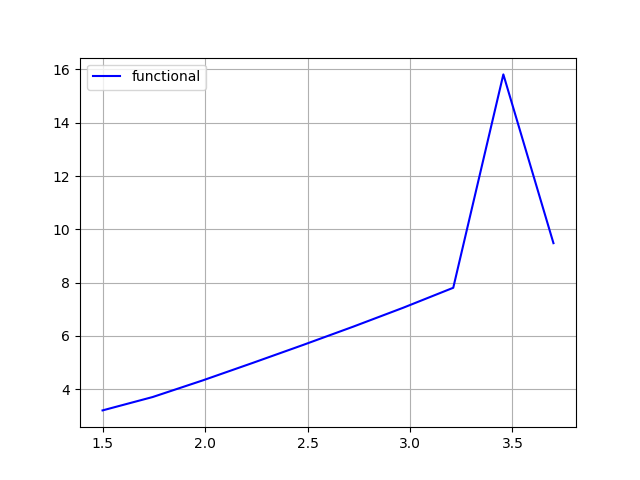
\includegraphics[scale=0.7]{fig/functional_1_5-3_7_50.png}
\caption{}
\end{figure}

\begin{figure}[H]
\center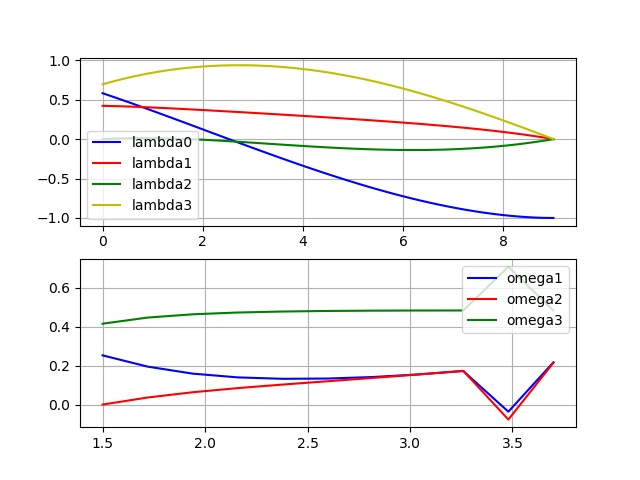
\includegraphics[scale=0.7]{fig/ivp_and_control_1_5-3_7_50.png}
\caption{}
\end{figure}

2 случай - зафиксировали $\alpha_1$ и $\alpha_2$, изменяли $\alpha_3$ на отрезке от $3.7$ до $5$ для случая малого угла в $5^{\circ}$.

Изображены в соответствии с рисунком 6.3 и с рисунком 6.4.

\begin{figure}[H]
\center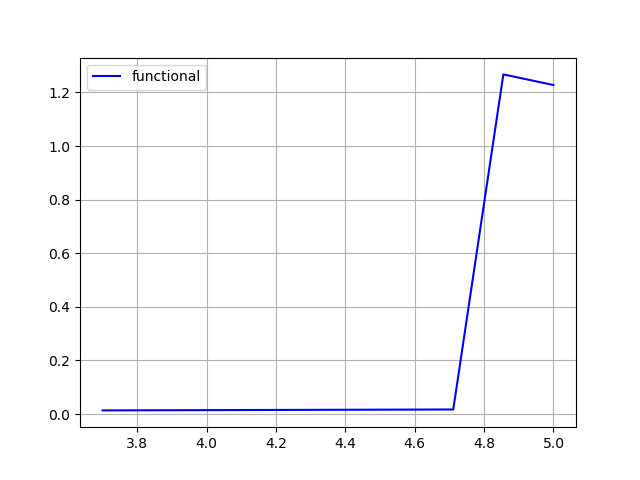
\includegraphics[scale=0.7]{fig/functional_3_7-5_5.png}
\caption{}
\end{figure}

\begin{figure}[H]
\center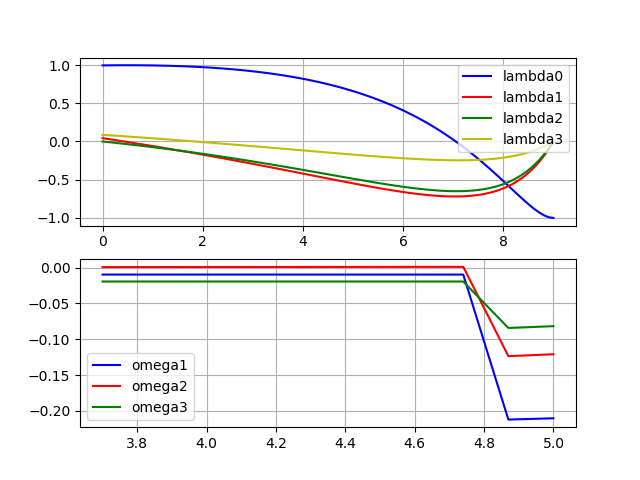
\includegraphics[scale=0.7]{fig/ivp_and_control_3_7-5_5.png}
\caption{}
\end{figure}

3 случай - зафиксировали $\alpha_1$ и $\alpha_3$, изменяли $\alpha_2$ на отрезке от $1.5$ до $3.7$ для случая большого угла в $50^{\circ}$.

При увеличение весового множителя $\alpha_2$ функционал $I$ имеет локальные минимумы в районе $1.7$ и $2.1$. От $2.4$ до $3$ происходит снижение расхода топлива. $\omega_1$ и $\omega_3$ уменьшается, а $\alpha_2$ увеличивается до $3.0$. После $3.0$ $\omega_1$, $\omega_2$ и $\omega_3$ не изменяются.

Изображены в соответствии с рисунком 6.5 и с рисунком 6.6.

\begin{figure}[H]
\center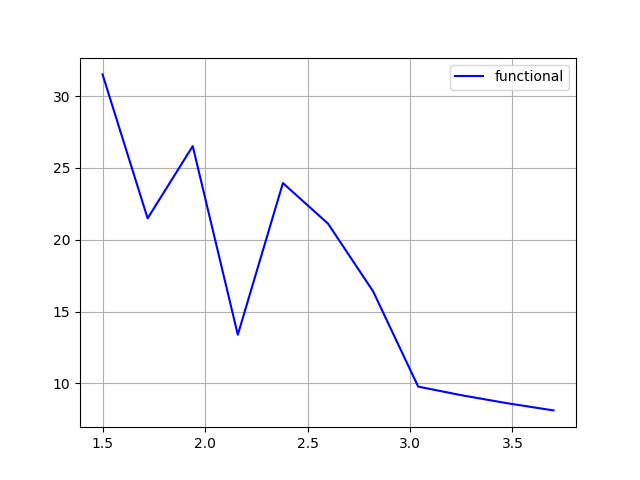
\includegraphics[scale=0.7]{fig/functional_alpha2_1_5-3_7_50.png}
\caption{}
\end{figure}

\begin{figure}[H]
\center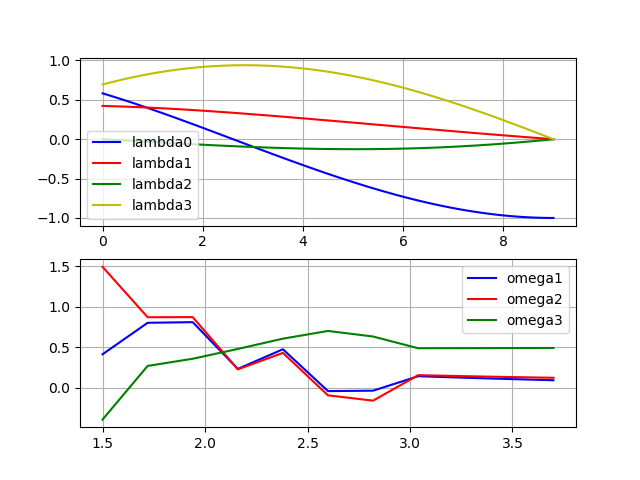
\includegraphics[scale=0.7]{fig/ivp_and_control_alpha2_1_5-3_7_50.png}
\caption{}
\end{figure}

4 случай - зафиксировали $\alpha_1$ и $\alpha_2$, изменяли $\alpha_3$ на отрезке от $1$ до $2$ для случая малого угла в $5^{\circ}$.

При увеличение весового множителя $\alpha_3$ функционал $I$ вначале растёт до $1.3$, потом уменьшается от $1.6$ и достигает своего минимума при $\alpha_3 = 1.9$. Увеличивая весовой множитель $\alpha_3$ в функционале $I$, $\omega_3$ уменьшается.

Изображены в соответствии с рисунком 6.7 и с рисунком 6.8.

\begin{figure}[H]
\center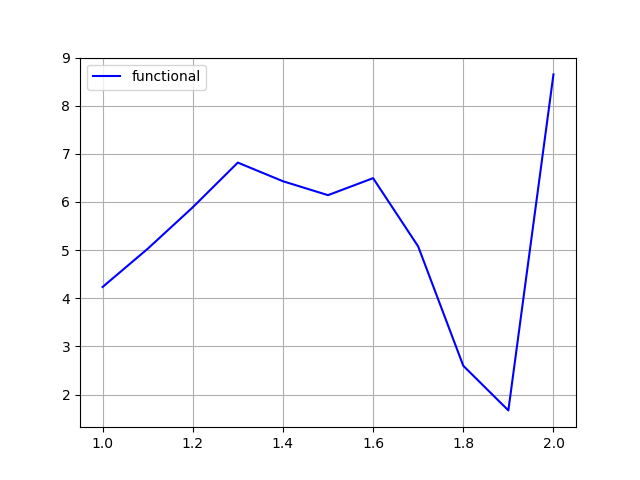
\includegraphics[scale=0.7]{fig/functional_alpha2_1-2_5.png}
\caption{}
\end{figure}

\begin{figure}[H]
\center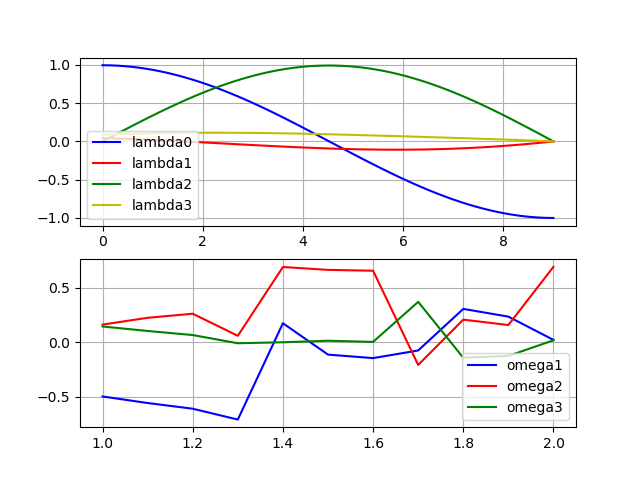
\includegraphics[scale=0.7]{fig/ivp_and_control_alpha2_1-2_5.png}
\caption{}
\end{figure}

\chapter{Разработка базы данных для хранения информации о проведённых экспериментах}
\section{Нереляционные хранилища данных}
Понятие NoSQL (Not Only SQL или No SQL) получило известность с 2009 года. Именно тогда развитие web-технологий и социальных сервисов дало толчок множеству новых подходов к хранению и обработке данных. Разработчики таких приложений столкнулись с задачами, для которых традиционные реляционные СУБД оказались либо слишком дороги, либо недостаточно производительны. Кроме того, популяризаторами отказа от универсальных «комбайнов» (реляционные СУБД – РСУБД) в пользу специализированных решений стали стартаперы и те, кому приходится работать в сценариях так называемых Big Data. Надо понимать, что NoSQL- решения не обязательно означают замену и полный отказ от РСУБД. Как обычно, инструмент должен выбираться под задачу, а не наоборот.

Когда говорят о NoSQL, обычно первым выделяют такое достоинство, как масштабируемость. Горизонтальное масштабирование существующих традиционных СУБД обычно является трудоемкой, дорогостоящей и эффективной только до определенного уровня задачей. В то же время многие NoSQL-решения проектировались исходя из необходимости масштабироваться горизонтально и делать это «на лету». Поэтому эта процедура обычно проще и прозрачнее в NoSQL, чем в РСУБД. Производительность БД на одном узле, а не в кластере также является немаловажным параметром. Для многих задач такие свойства традиционных СУБД, как транзакционность, изолированность изменений, надежность в пределах одного узла или даже сама реляционная модель, не всегда нужны в полном объеме. Поэтому отказ от этих свойств (всех или некоторых) позволяет NoSQL иногда добиваться большей производительности на одном узле, чем традиционным решениям. Надежная работа в условиях, когда отказ железа или сетевая недоступность – обычное дело, является одним из свойств многих решений NoSQL. Основной способ ее обеспечения – это репликация. Сама по себе репликация отнюдь не является уникальной особенностью NoSQL, но здесь, как и при масштабировании, важную роль играют эффективность и легкость внесения изменений в существующую инсталляцию. Переход БД к работе в режиме репликации – это простая задача для большинства NoSQL-решений. Простота разработки и администрирования – также важный аргумент в пользу NoSQL-технологий.
Целый ряд задач, связанных с масштабированием и репликацией, представляющих значительную сложность и требующих обширной специальной экспертизы на традиционных СУБД, у NoSQL занимает считанные минуты. Задачи установки и настройки, само использование NoSQL-решений обычно существенно проще и менее трудоемки, чем в случае с РСУБД. Поэтому NoSQL-системы стали очевидным выбором для многих стартапов, где скорость разработки и внедрения является ключевым фактором.

\section{СУБД MongoDB}
Первая публичная версия MongoDB была выпущена в 2009 году, а теперь это восходящая звезда в мире NoSQL. Система задумывалась как масштабируемая база данных – название Mongo происходит от слова «humongous», получившегося объединением «huge» (гигантский) и «monstrous» (чудовищный), а в качестве основных проектных целей были поставлены высокая производительность и простота доступа к данным. Это документная база данных, которая позволяет не только хранить, но и опрашивать вложенные данные, предъявляя произвольные запросы. Схема базы данных не навязывается (в этом MongoDB похожа на Riak, но отличается от Postgres), поэтому один
документ может содержать поля или типы, отсутствующие во всех остальных документах коллекции \cite{mongodb}.

Mongo счастливо сочетает в себе мощные средства запросов, характерные для реляционных баз данных, и распределенную архитектуру, свойственную таким хранилищам, как Riak или HBase. Mongo – хранилище JSON-документов (хотя, строго говоря, данные хранятся в двоичном варианте JSON, который называется BSON). BSON позволяет работать с данными быстрее: быстрее выполняется поиск и обработка. Хотя надо отметить, что BSON в отличие от хранения данных в формате JSON имеет небольшой недостаток: в целом данные в JSON-формате занимают меньше места, чем в формате BSON, с другой стороны, данный недостаток с лихвой окупается скоростью. Документ Mongo можно уподобить строке реляционной таблицы без схемы, в которой допускается произвольная глубина вложенности значений. JSON-документ, изображённый в соответствии с рисунком 7.1.
\begin{figure}[H]
\center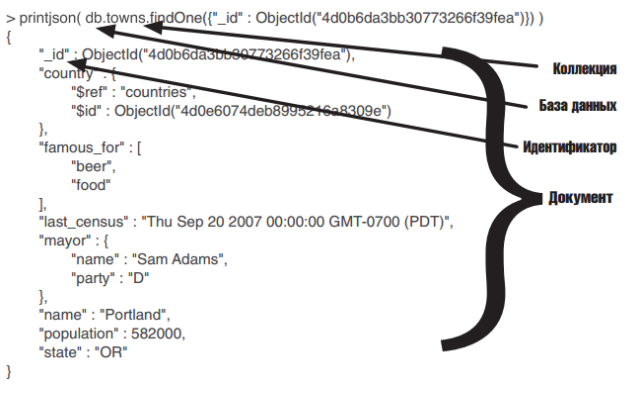
\includegraphics[scale=0.75]{fig/img81.png}
\caption{Пример JSON-документа}
\end{figure}

Документ можно представить как хранилище ключей и значений. Ключ представляет простую метку, с которым ассоциирован определенный кусок данных. Однако при всех различиях есть одна особенность, которая сближает MongoDB и реляционные базы данных. В реляционных СУБД встречается такое понятие как первичный ключ. Это понятие описывает некий столбец, который имеет уникальные значения. В MongoDB для каждого документа имеется уникальный идентификатор, который называется \_id. И если явным образом не указать его значение, то MongoDB автоматически сгенерирует для него значение. Каждому ключу сопоставляется определенное значение. Но здесь также надо учитывать одну особенность: если в реляционных базах есть четко очерченная структура, где есть поля, и если какое-то поле не имеет значение, ему (в зависимости от настроек конкретной базы данных) можно присвоить значение NULL. В MongoDB все иначе. Если какому-то ключу не сопоставлено значение, то этот ключ просто опускается в документе и не употребляется.

Вся система MongoDB может представлять не только одну базу данных, находящуюся на одном физическом сервере. Функциональность MongoDB позволяет расположить несколько баз данных на нескольких физических серверах, и эти базы данных смогут легко обмениваться данными и сохранять целостность.

\section{Результаты вычислений}
Были построены графики оптимального управления с разными весовыми множителями в минимизирующем функционале, которые переводят твердое тело из начального углового положения \eqref{init-angular-position} в конечное положение \eqref{fin-angular-position} и доставляющее минимум функционалу \eqref{min-functional}, который характеризует расход топлива на переориентацию тела \cite{samarskii}.

Изображения графиков функций оптимального управления, угловых скоростей и функционалов сериализуются и сохраняются как BLOB в базу данных MongoDB, а также массивы значений этих функций в разные моменты времени сохраняются.

\conclusions

Решена задача оптимальной переориентации твердого тела. Была сведена задача оптимальной переориентации твердого тела с помощью принципа максимума Л.С. Понтрягина к решению краевой задачи для системы обыкновенных дифференциальных уравнений \eqref{system-2ODU} с краевыми условиями \eqref{init-angular-position}, \eqref{fin-angular-position} \cite{vasileva}.
 
Для решения задачи применены решатели odeint и fsolve из библиотеки SciPy \cite{lutz}. Изображения графиков функций оптимального управления, угловых скоростей и функционалов сериализуются и сохраняются как BLOB в базу данных MongoDB, а также массивы значений этих функций в разные моменты времени сохраняются.

\bibliographystyle{utf8gost780u}
\nocite{*}
\bibliography{biblio}

\Appendix

\chapter{Исходный код реализации}
Исходный код реализации хранится в Github репозитории и доступен по ссылке: \href{https://github.com/titoffag/diploma}{https://github.com/titoffag/diploma}

\end{document}
